% FIXME: Stick to a naming convention, and disambiguate!
% Resolve:
% - pseudometabolite/bulk metabolite/biomass component/macromolecule
%   --> biomass component metabolite (some aren't macromolecules, e.g. ions)
% - pseudoreaction/isa reaction
%   --> isa reaction (pseudoreaction is too broad, isa reaction introduced in Yeast5),
%   then use biomass component-generating isa reaction
% - biomass reaction/growth reaction/objective function
%   --> prefer biomass reaction
% - use of the term 'flux', esp. 'flux through reaction'
% FIXME: Check if g/mol units for molecular weights of biomass makes sense
% (should it be g/mmol?)
\chapter{Modelling the yeast metabolic cycle}
\label{ch:model}

It is difficult to develop a fine-grained model for the aspects of the YMC,
especially if most of the molecular mechanisms are unclear
and if the main read-outs of single-cell studies --- NAD(P)H and flavins autofluorescence --- are `aggregate' measures of several biochemical phenomena.
It is perhaps more feasible to construct coarse-grained models to answer specific biological questions with the YMC.
Here, I present using a genome-scale metabolic model and flux balance analysis (FBA) to address the logic of the metabolic cycle.
Specifically, why is it advantageous for the cell, and is it linked to resource allocation?

\section{Introduction to flux balance analysis}
\label{sec:model-fba}

TODO: Short introduction to genome-scale metabolic models -- what they are, what they aim to do, flux balance analysis, and limitations.

\section{Reviewing modelling temporal partitioning of biosynthesis}
\label{sec:model-temporal}

In this chapter, my research question with modelling the temporal partitioning of biosynthesis is:
does a finite enzyme pool explain metabolic cycling or temporal segregation of biomass components --- lipids, carbohydrates, amino acids, nucleic acids --- in the YMC?
If so, can the model predict the dependence of the time scale on nutrient conditions?
Additionally, does such a time scale fit with that of the YMC?

Previous studies have attempted to address differing metabolic requirements in each phase of the yeast metabolic cycle using flux balance analysis (FBA).
\textcite{takhaveevTemporalSegregationBiosynthetic2023} showed that in different stages of the cell division cycle, the level of synthesis of each class of macromolecule is different.
They blocked synthesis of each class of macromolecule and recorded the changes in single-cell NAD(P)H cycles, representing the YMC, to build a picture of the temporality of the biosynthesis of macromolecules over a cell division cycle.
Then, they used these activities as coefficients for FBA on a modified thermodynamic-stoichiometric metabolic model at each time point to deduce biomass production rates.
% Does not suggest that synthesis of each class of macromolecule excludes all others (which makes sense).
% Rather, this study confirms that timescale of observed synthesis events matches simulations.
% Do I even cite this?  It's so bad.
Additionally, \textcite{cesurGenomeWideAnalysisYeast} constructed a different FBA model for each YMC phase based on transcriptomic and epigenetic data, using the GIMME algorithm, which excludes reactions that correspond to genes that are not expressed at certain time points.
Both studies model behaviours at each phase of the YMC, rather than predicting timescale.

An attempt in extending FBA to solve a time-dependent resource allocation problem was \textcite{reimersCellularTradeoffsOptimal2017}, in which they extend a genome-scale model of the cyanobacterium \textit{Synechococcus elongatus} PCC7942 to address the temporal order of intracellular synthesis reactions that optimises the growth rate of the cell, under resource constraints.
However, this model relies on an external oscillation --- namely, the light-dark cycle --- in contrast to the yeast metabolic cycle which is autonomously generated.
Therefore, this study has limited applicability to my study.

I use a genome-scale model of \textit{Saccharomyces cerevisiae} and perform flux balance analysis (FBA).
Specifically, I use the enzyme-constrained Yeast8 (ecYeast8) model \parencite{luConsensusCerevisiaeMetabolic2019}.
I use this model because it is the most recent, offering a good coverage of reactions, and is continuously updated in a well-characterised and well-documented software repository.
Here, I use models Yeast8.6.0 and ec\-Yeast\-8.6.0, the latest version for which both original and enzyme-constrained variants are available.
In addition, it has `pseudometabolites' defined by \textit{isa} reactions \parencite{heavnerYeastExpandedReconstruction2012} that group specific chemical species in general classes, making it easy to study each class of biomass component (e.g. lipid, protein, carbohydrate) individually.

Traditional genome-scale models assume that the uptake rate of carbon source limits production.
However, levels of each enzyme also restrict reaction fluxes, leading to the development of enzyme-constrained models.
An enzyme-constrained model fits the assumption that there is a fixed number of amino acids the cell has to distribute \parencite{weisseMechanisticLinksCellular2015}.
Models like \textcite{sanchezImprovingPhenotypePredictions2017} and \textcite{elsemmanWholecellModelingYeast2022} --- the latter of which imposes a ribosome capacity constraint and additionally imposes compartment constraints --- constrain the total sum of fluxes based on a defined total amount of enzyme.
ecYeast8 uses the GECKO formalism \parencite{sanchezImprovingPhenotypePredictions2017}, specifically GECKO 2 \parencite{domenzainReconstructionCatalogueGenomescale2022}, which applies the enzyme constraint by modifying the stoichiometric matrix of a genome-scale metabolic model.

\section{The Yeast8 and ecYeast8 models and their formalisms}
\label{sec:model-yeast8}

In this section, I discuss the formalisms used in ecYeast8 because they differ from the usual formalisms used in other genome-scale metabolic models and because I take advantage of some of these formalisms.

ecYeast8 contains four formalisms relevant to my study:
\begin{enumerate}
  \item
        The biomass reaction is defined by having `pseudometabolites' as reactants and a biomass species as a product.
        These pseudometabolites include lipids, proteins, carbohydrates, RNA, DNA, ions, and cofactors.
        This is in contrast to BiGG genome-scale models that have biomass reactions defined by having chemical species as reactants, each with a stoichiometric coefficient representing the species' abundance in units of \SI{}{\milli\mol~\gram_{DW}^{-1}}.
  \item
        The pseudometabolites are defined by `\textit{isa}' reactions, which group specific chemical species into classes of metabolites.
        This accounts for some KEGG definitions of reactions requiring generic compounds and allows flexibility of biomass definition in different growth conditions.
        These \textit{isa} reactions are defined by having chemical species as reactants, each with a stoichiometric coefficient representing the species' abundance in units of \SI{}{\milli\mol~\gram_{DW}^{-1}}, and a pseudometabolite as a product.
        In effect, the abundances are shifted one reaction away from the biomass reaction.
  \item
        SLIMEr \parencite{sanchezSLIMErProbingFlexibility2019}, which Splits Lipids Into Measurable Entities, and adds constraints on lipid classes and acyl chain distribution.
        This formalism, specifically for lipid metabolism, is needed because species of lipid backbones and acyl chain can combine to form lipids in more than a thousand ways, and the resulting lipid species are difficult to all be accounted for in a genome-scale metabolic model.
        SLIMEr thus introduces reactions that split lipids into their basic components and lipid pseudoreactions to preserve the distribution of acyl chains.
        The result is that the definitions of lipids are flexible.
  \item
        GECKO was applied to Yeast8 to produce ecYeast8.  GECKO modifies the stoichiometric matrix of an input genome-scale metabolic model to account for enzyme abundances and kinetics.
        Specifically, it adds to enzyme-catalysed reactions enzyme species with a stoichiometric coefficient derived from its $k_{cat}$ value.
        The formalism also adds reactions to model drawing enzymes from a pool.  GECKO models the case where there is an upper limit of the amount of amino acids available to be allocated to enzyme production.
\end{enumerate}

Here, I detail how I apply these formalisms for my study.
% TODO: Use proper refs rather than hard-coding numbers.
These all affect my study, but I detail in particular GECKO (item 4) and computing molecular weights of pseudometabolites (based on items 1 and 2).

% FIXME: Delete this subsection?
% It's mostly a duplicate of the appendix of the GECKO paper,
% and I wrote it just to make sure I understand it.
% I haven't used it in discussion so far.
% FIXME: CHECK FOR PLAGIARISM!!!
\subsection{GECKO}
\label{subsec:model-yeast8-gecko}

ecYeast8 is derived from Yeast8 by applying the GECKO formalism.
In a conventional genome-scaled model, metabolic fluxes through reactions are constrained between a lower bound and an upper bound.
This constraint narrows down the solution space when the objective function is optimised.
GECKO imposes an additional constraint on the metabolic fluxes based on the concentration of the enzyme that catalyses the reaction.
As a simple example, for a reaction $R_{j}$ catalysed by enzyme $E_{i}$ (and $E_{i}$ only), the formalism imposes:

\begin{equation}
  v_{j} \leq k_{\mathrm{cat}}^{ij} \cdot [E_{i}]
  \label{eq:model-gecko-kcat}
\end{equation}

In other words, the flux through the reaction must not exceed $v_{\mathrm{max}}$.
Slightly different relationships are imposed for other types of enzymes, i.e. isozymes, promiscuous enzymes, and enzyme complexes.

To apply this constraint, GECKO modifies reactions in the genome-scaled model it is applied to.
For example, if the model defines a reaction $R_{j}$ catalysed by $E_{i}$:
\begin{equation}
  \ce{ A + B ->[E_{i}] C + D }
  \label{eq:model-gecko-catalysed}
\end{equation}

GECKO adds a term to the equation, modifying the stoichiometric matrix, to make it:
\begin{equation}
  \ce{ n_{ij}E_{i} + A + B -> C + D }
  \label{eq:model-gecko-catalysed-formalism}
\end{equation}
with $n_{ij} = \frac{1}{k_{\mathrm{cat}}^{ij}}$.
This transformation, adding the enzyme as a pseudo-reactant, is based on the interpretation that the system uses some amount of enzyme at a specific time to catalyse the flux going through the reaction.

% GECKO then also creates an overall enzyme pseudo-reaction $EU_{i}$: $\ce{ -> E_{i}}$, in order to preserve the mass balance of enzymes.  The flux $e_{i}$ of this pseudo-reaction is thus constrained: $0 \le e_{i} \le [E_{i}]$.

Slightly different formalisms are applied to reversible reactions, isozymes, promiscuous enzymes, and enzyme complexes.  Namely:
\begin{itemize}
  \item Reversible reactions are modelled as the forward and reverse reactions separately.
  \item For isozymes, the original reaction is copied $n$ times corresponding to the number of reactions that the isozyme catalyses. Each has an isozyme catalysing the reaction.
  In addition, there is an `arm' reaction to act as an intermediate between the substrate and the products.
  \item No actions are needed for promiscuous enzymes.
  \item Enzyme complexes are modelled as one reaction that uses all subunit proteins that all share the same $k_{cat}$ value.
\end{itemize}

GECKO repeats this logic for all enzyme-catalysed reactions in the genome-scale model to create an enzyme-constrained model.
GECKO takes $k_{cat}$ values from BRENDA \parencite{changBRENDAELIXIRCore2021} and enzyme data from SWISSPROT \parencite{theuniprotconsortiumUniProtUniversalProtein2023} and KEGG \parencite{kanehisaKEGGTaxonomybasedAnalysis2023}, including molecular weight of protein and associated pathways.

To constrain enzyme levels in the model, GECKO defines a pseudo-reaction

\begin{equation}
  ER_{\mathrm{pool}}: \varnothing \ce{ -> E_{pool} }
  \label{eq:model-gecko-enzyme-pool}
\end{equation}

with a flux $e_{\mathrm{pool}} \leq (P_{\mathrm{total}} - P_{\mathrm{measured}}) \cdot f \cdot \sigma$ in units of \SI{}{\gram~\gram_{DW}^{-1}}, where

\begin{itemize}
  \item $P$ represents protein fraction with respect to the dry weight of the cell,
  \item $f$ represents the fraction of proteins that are enzymes, and
  \item $\sigma$ is a parameter that represents the average saturation of enzymes.
\end{itemize}

ecYeast8.6.0 assumes parameter values of: $f = 0.5$, $P_{\mathrm{total}} = 0.5$, and $\sigma = 0.5$.
Defining such parameters is a judgement call, especially when the protein fraction varies across growth rates, but $f = 0.5$ is close to the model's mass fraction (to be discussed in section~\ref{subsec:model-yeast8-molweights}).
Subsequently, GECKO changes the carbohydrate composition based on the assumption that a change in the amino acid composition is offset by the reverse change in the carbohydrate composition;
experimental data justifies this assumption.

Then, for each enzyme $\ce{E_{i}}$, GECKO defines enzyme usage pseudo-reactions of the form

\begin{equation}
  ER_{i}: \ce{ MW_{i} E_{\mathrm{pool}} -> E_{i} }
  \label{eq:model-gecko-enzyme-usage}
\end{equation}

with $MW_{i}$ being the molecular weight of the enzyme in units of \SI{}{\gram~\milli\mole^{-1}}.
The flux of enzyme usage pseudo-reactions are defined in units of \SI{}{\milli\mole~\gram_{DW}^{-1}}.
Taken together, the modelled cell thus has an enzyme pool in terms of a mass fraction of the cell's dry weight, and the modelled cell allocates certain fractions of this mass to the synthesis of each enzyme at steady-state.  The mass of each enzyme in the cell determines the amount (moles) of each enzyme and therefore its catalytic activity.

\subsection{Computing molecular weights of pseudometabolites}
\label{subsec:model-yeast8-molweights}

In the yeast cell, biomass components (lipids, carbohydrates, proteins) are present in different fractions.
Knowing these fractions are useful in computing the time it takes to synthesise each biomass component (to be discussed later).
As discussed in section~\ref{sec:model-yeast8}, these fractions are represented in the biomass reaction.
However, the mass fraction of each component varies according to strain and growth rate \parencite{nilssonMetabolicTradeoffsYeast2016, elsemmanWholecellModelingYeast2022}.
It is not straightforward to implement these changes as stoichiometric coefficients of individual species that define biomass, because there is limited detailed information for the mass fractions of such species as conditions vary, and because of the many combinations of lipid backbones and acyl chains.
Therefore, I decided to compute the mass fractions of each biomass component based on the stoichiometries of species in the Yeast8 model, as a back-of-the-envelope calculation for such a coarse-grained modelling effort.
Similar calculations were performed by \parencite{takhaveevTemporalSegregationBiosynthetic2023}.

\textit{isa} reactions define pseudometabolites by having chemical species with known molecular weights as reactants, with their stoichiometric coefficients representing abundance in \SI{}{\milli\mol~\gram_{DW}^{-1}}.
Therefore, I can treat each pseudometabolite as a chemical species and calculate its molecular weight by assuming mass balance \parencite{chanStandardizingBiomassReactions2017, dinhQuantifyingPropagationParametric2022, takhaveevTemporalSegregationBiosynthetic2023};
the resulting molecular weight will thus represent the mass fraction of each biomass component in units of \SI{}{\gram~\gram_{DW}^{-1}}.

For this to be possible, I needed to compute molecular weights for bulk metabolites that represent macromolecules in the ecYeast8 model.
The ecYeast8 model does not specify the molecular weights of these bulk metabolites.
The bulk metabolites includes: lipids (\texttt{s\_1096}), proteins (\texttt{s\_3717}), carbohydrates (\texttt{s\_3718}), RNA (\texttt{s\_4049}), and DNA (\texttt{s\_3720}).
Additionally, I computed molecular weights for bulk metabolites that represent cofactors (\texttt{s\_4205}), and ions (\texttt{s\_4206}), as they are part of the objective function too.
Namely, I assumed that in reactions that produce the bulk metabolites, there is conservation of mass, and therefore:

\begin{equation}
\label{eq:conservation-of-mass}
  \begin{aligned}
    \sum_{s}(\text{molar mass}_{s})(\text{stoichiometric coefficient}_{s}) \\ = \sum_{p}(\text{molar mass}_{p})(\text{stoichiometric coefficient}_{p})
  \end{aligned}
\end{equation}

where $s = 1, ...$ \emph{(number of substrates)} represents substrates and $p = 1, ...$ \emph{(number of products)} represents products of the reaction in question.

To compute the molecular weight of the carbohydrate metabolite, I inspected reaction \texttt{r\_4048}:

\texttt{
  0.684535 (1->3)-beta-D-glucan + 0.228715 (1->6)-beta-D-glucan \\
  + 0.330522 glycogen + 0.650171 mannan + 0.126456 trehalose \\
  --> carbohydrate
}

Here, the molecular weights of all species except for \texttt{carbohydrate}, the bulk metabolite, are represented in the model.
Thus, equation \ref{eq:conservation-of-mass} can be applied to compute the molecular weight of the carbohydrate metabolite.

The same process can be applied to compute the molecular weights of the DNA, RNA, cofactor, and ion metabolites as the equations similarly have reactants with molecular weights represented in the model and only the bulk metabolite, the sole product, as the metabolite with an unspecified molecular weight.
The DNA molecular weight was computed from reaction \texttt{r\_4050}:

\texttt{
  0.0036 dAMP + 0.0024 dCMP + 0.0024 dGMP + 0.0036 dTMP \\
  --> DNA
}

The RNA molecular weight was computed from reaction \texttt{r\_4049}:

\texttt{
  0.0445348 AMP + 0.0432762 CMP + 0.0445348 GMP + 0.0579921 UMP \\
  --> RNA
}

The cofactor molecular weight was computed from reaction \texttt{r\_4598}:

\texttt{
  0.00019 coenzyme A + 1e-05 FAD + 0.00265 NAD + 0.00015 NADH \\
  + 0.00057 NADP(+) + 0.0027 NADPH + 0.00099 riboflavin \\
  + 1.2e-06 TDP + 6.34e-05 THF + 1e-06 heme a \\
  --> cofactor
}

And the ion molecular weight was computed from reaction \texttt{r\_4599}:

\texttt{
  3.04e-05 iron(2+) + 0.00363 potassium + 0.00397 sodium + 0.02 sulphate \\
  + 0.00129 chloride + 0.00273 Mn(2+) + 0.000748 Zn(2+) + 0.000217 Ca(2+) \\
  + 0.00124254 Mg(2+) + 0.000659 Cu(2+) \\
  --> ion
}

Other metabolites were less straightforward and required some judgement calls.
To compute the molecular weight of the protein metabolite, I inspected reaction \texttt{r\_4047}:

\texttt{
  0.57284 Ala-tRNA(Ala) + 0.200644 Arg-tRNA(Arg) + 0.126979 Asn-tRNA(Asn)\\
  + ... + 0.330369 Val-tRNA(Val) \\
  --> 0.57284 tRNA(Ala) + 0.200644 tRNA(Arg) + 0.126979 tRNA(Asn) \\
  + ... + 0.330369 tRNA(Val) + protein
}

In this reaction, the aminoacyl-tRNA reactants are represented in the form of the atoms that make up the aminoacyl residues plus \texttt{R} to represent the tRNA, and the tRNA products are represented as \texttt{RH}.
For example, \texttt{Ala-tRNA(Ala)}, alanyl-tRNA, is represented as \texttt{C3H7NOR}.
The protein pseudoreaction shows how different proportions of each aminoacyl-tRNA combine to form the cell's proteins, so it is safe to discard the \texttt{R} symbol that corresponds to the tRNA from the reaction.
On doing so, the mass balance represented by equation~\ref{eq:conservation-of-mass} can be applied to compute the molecular weight of the protein metabolite.

Finally, the lipid metabolite is the least straightforward because some of the reactants do not have molecular weights specified.
The lipid pseudoreaction is represented in reaction \texttt{r\_2108}:

\texttt{
  lipid backbone + lipid chain --> lipid
}

And both \texttt{lipid backbone} and \texttt{lipid chain} have no molecular weight specified.

Reaction \texttt{r\_4065} specifies a lipid chain pseudoreaction, in which \texttt{lipid chain} is generated:

\texttt{
  0.0073947 C16:0 chain + 0.0217019 C16:1 chain + 0.0020726 C18:0 chain \\
  + 0.000796243 C18:1 chain \\
  --> lipid chain
}

As all reactants have molecular weights defined in the model, the molecular weight of \texttt{lipid chain} can be computed from the mass balance of this reaction.

Reaction \texttt{r\_4063} specifies a lipid backbone pseudoreaction, in which \texttt{lipid backbone} is generated:

\texttt{
  0.000631964 1-phosphatidyl-1D-myo-inositol backbone\\
  + 0.00243107 ergosterol + 0.000622407 ergosterol ester backbone\\
  + 0.000135359 fatty acid backbone + ...\\
  --> lipid backbone
}

Within this reaction, all reactants have defined molecular weights except for \texttt{fatty acid backbone}.
Because of SLIMEr, four reactions in the model produce \texttt{fatty acid backbone}:
\begin{table}[ht]
  \centering
    \begin{tabular}{llS}
      ID & Reaction & {\makecell{Computed molecular\\ weight (\SI{}{\gram~\mole^{-1}})}} \\
      \hline
    \texttt{r\_3975} & \makecell{\texttt{palmitate} \\ \texttt{--> 0.255421 fatty acid backbone} \\ \texttt{0.256429 C16:0 chain}} & 742.54 \\
    \texttt{r\_3976} & \makecell{\texttt{palmitoleate} \\ \texttt{--> 0.253405 fatty acid backbone} \\ \texttt{0.254413 C16:1 chain}} & 744.56 \\
    \texttt{r\_3977} & \makecell{\texttt{stearate} \\ \texttt{--> 0.283475 fatty acid backbone} \\ \texttt{0.284483 C18:0 chain}} & 714.49 \\
    \texttt{r\_3978} & \makecell{\texttt{oleate} \\ \texttt{--> 0.281459 fatty acid backbone} \\ \texttt{0.282467 C18:1 chain}} & 716.51 \\
    \end{tabular}
    \caption{ecYeast8 reactions that generate the \texttt{fatty acid backbone} metabolite}
    \label{tab:ecyeast8-fatty-acid-backbone-rxns}
\end{table}

All species in these reactions except for \texttt{fatty acid backbone} have molecular weights specified, and thus I applied mass balance to find the molecular weight of \texttt{fatty acid backbone} from each reaction.
However, the molecular weights computed from each equation are different, as shown in the table above.
Since the differences are slight, and ultimately I am making a back-of-the-envelope calculation, I took the mean of the four weights (\SI{729.53}{\gram~\mole^{-1}}) as the molecular weight of \texttt{fatty acid backbone} for the purposes of computing the molecular weight of \texttt{lipid backbone} (which then yields \SI{21.31}{\gram~\mole^{-1}}).

With the molecular weights of \texttt{lipid backbone} and \texttt{lipid chain} defined, I can now compute the molecular weight of \texttt{lipid} using mass balance.

In summary, the molecular weights of the bulk metabolites are:
\begin{table}[ht]
  \centering
  \begin{tabular}{lS}
    Metabolite & {Computed molecular weight (\SI{}{\gram~\mol^{-1}})} \\
    \hline
    Protein & 504.37 \\
    Carbohydrate & 350.37 \\
    RNA & 64.04 \\
    Lipid & 31.57 \\
    Cofactors & 4.83 \\
    DNA & 3.90 \\
    Ions & 2.48
  \end{tabular}
  \caption{Computed molecular weights of bulk metabolites in ecYeast8}
  \label{tab:ecyeast8-mol-weights}
\end{table}

As additional validation, the ratio between the molecular weights are similar to the ratio between the mass of each class of macromolecule in the yeast cell dry weight shown by \textcite{canelasVivoDatadrivenFramework2011}.

And thus the molecular weight of biomass is \SI{961.57}{\gram~\mol^{-1}}, close to the \SI{966}{\gram~\mol^{-1}} in \textcite{takhaveevTemporalSegregationBiosynthetic2023} computed from a different genome-scale model.
In theory, this number should be \SI{1000}{\gram~\mol^{-1}} because the stoichiometric coefficients of the species that form biomass components are expressed in terms of \SI{}{\milli\mol~\gram_{DW}^{-1}} \parencite{thieleProtocolGeneratingHighquality2010, palssonSystemsBiologyConstraintbased2015}, but the slight deviation from 1000 could be explained by the SLIMEr formalism.
Plus, it has been reported that the sum of stoichiometric coefficients are not always verified \parencite{chanStandardizingBiomassReactions2017}.

% Could move to 'results' part of this chapter?
\section{Ablating pseudometabolites from the biomass reaction}
\label{sec:model-yeast8-pseudometabolites}

To simulate producing each class of biomass component in turn,
I take advantage of pseudometabolites in ecYeast8 to remove each of them in turn from the biomass reaction ---
in other words, ablating pseudometabolites from the biomass reaction.
Specifically, I exclude each pseudometabolite in turn in the objective function (biomass-generating reaction) and optimise the model.

Given the objective function:

\texttt{
  47.5883 atp\_c + 47.5883 h2o\_c + lipid\_c + protein\_c + carbohydrate\_c\\
  + dna\_c + rna\_c + cofactor + ion \\
  --> 47.5883 adp\_c + biomass\_c + 47.5883 h\_c + 47.5883 pi\_c
}

There are seven pseudometabolites: lipids, proteins, carbohydrates, DNA, RNA, cofactor, and ion.
To have the cell prioritise biosynthesis of lipids, I set the stoichiometries of all five classes except for lipids to zero in the above equation, giving:

\texttt{
  47.5883 atp\_c + 47.5883 h2o\_c + lipid\_c + cofactor + ion \\
  --> 47.5883 adp\_c + biomass\_c + 47.5883 h\_c + 47.5883 pi\_c
}

And I repeated this for the other pseudometabolites.

\begin{figure}
  \centering
  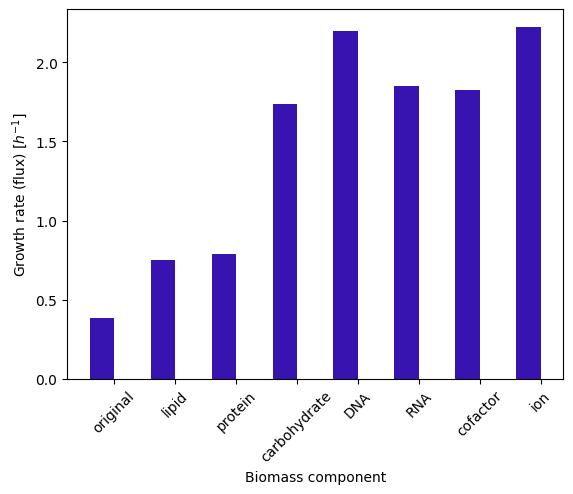
\includegraphics[width=.9\linewidth]{ablation_example_fluxes.png}
  \caption{
    Growth rates, from fluxes of the biomass reaction, from the original wild type model ($\lambda_{0}$; leftmost bar) and from the ablated versions of the model ($\lambda_{i}^{\prime}$, where $i$ represents each biomass components among lipids, proteins, carbohydrates, DNA, RNA, cofactors, and ions; other bars)
  }
  \label{fig:model-ablate-fluxes}
\end{figure}

I get modified growth rates as in figure~\ref{fig:model-ablate-fluxes}.

\begin{figure}
  \centering
  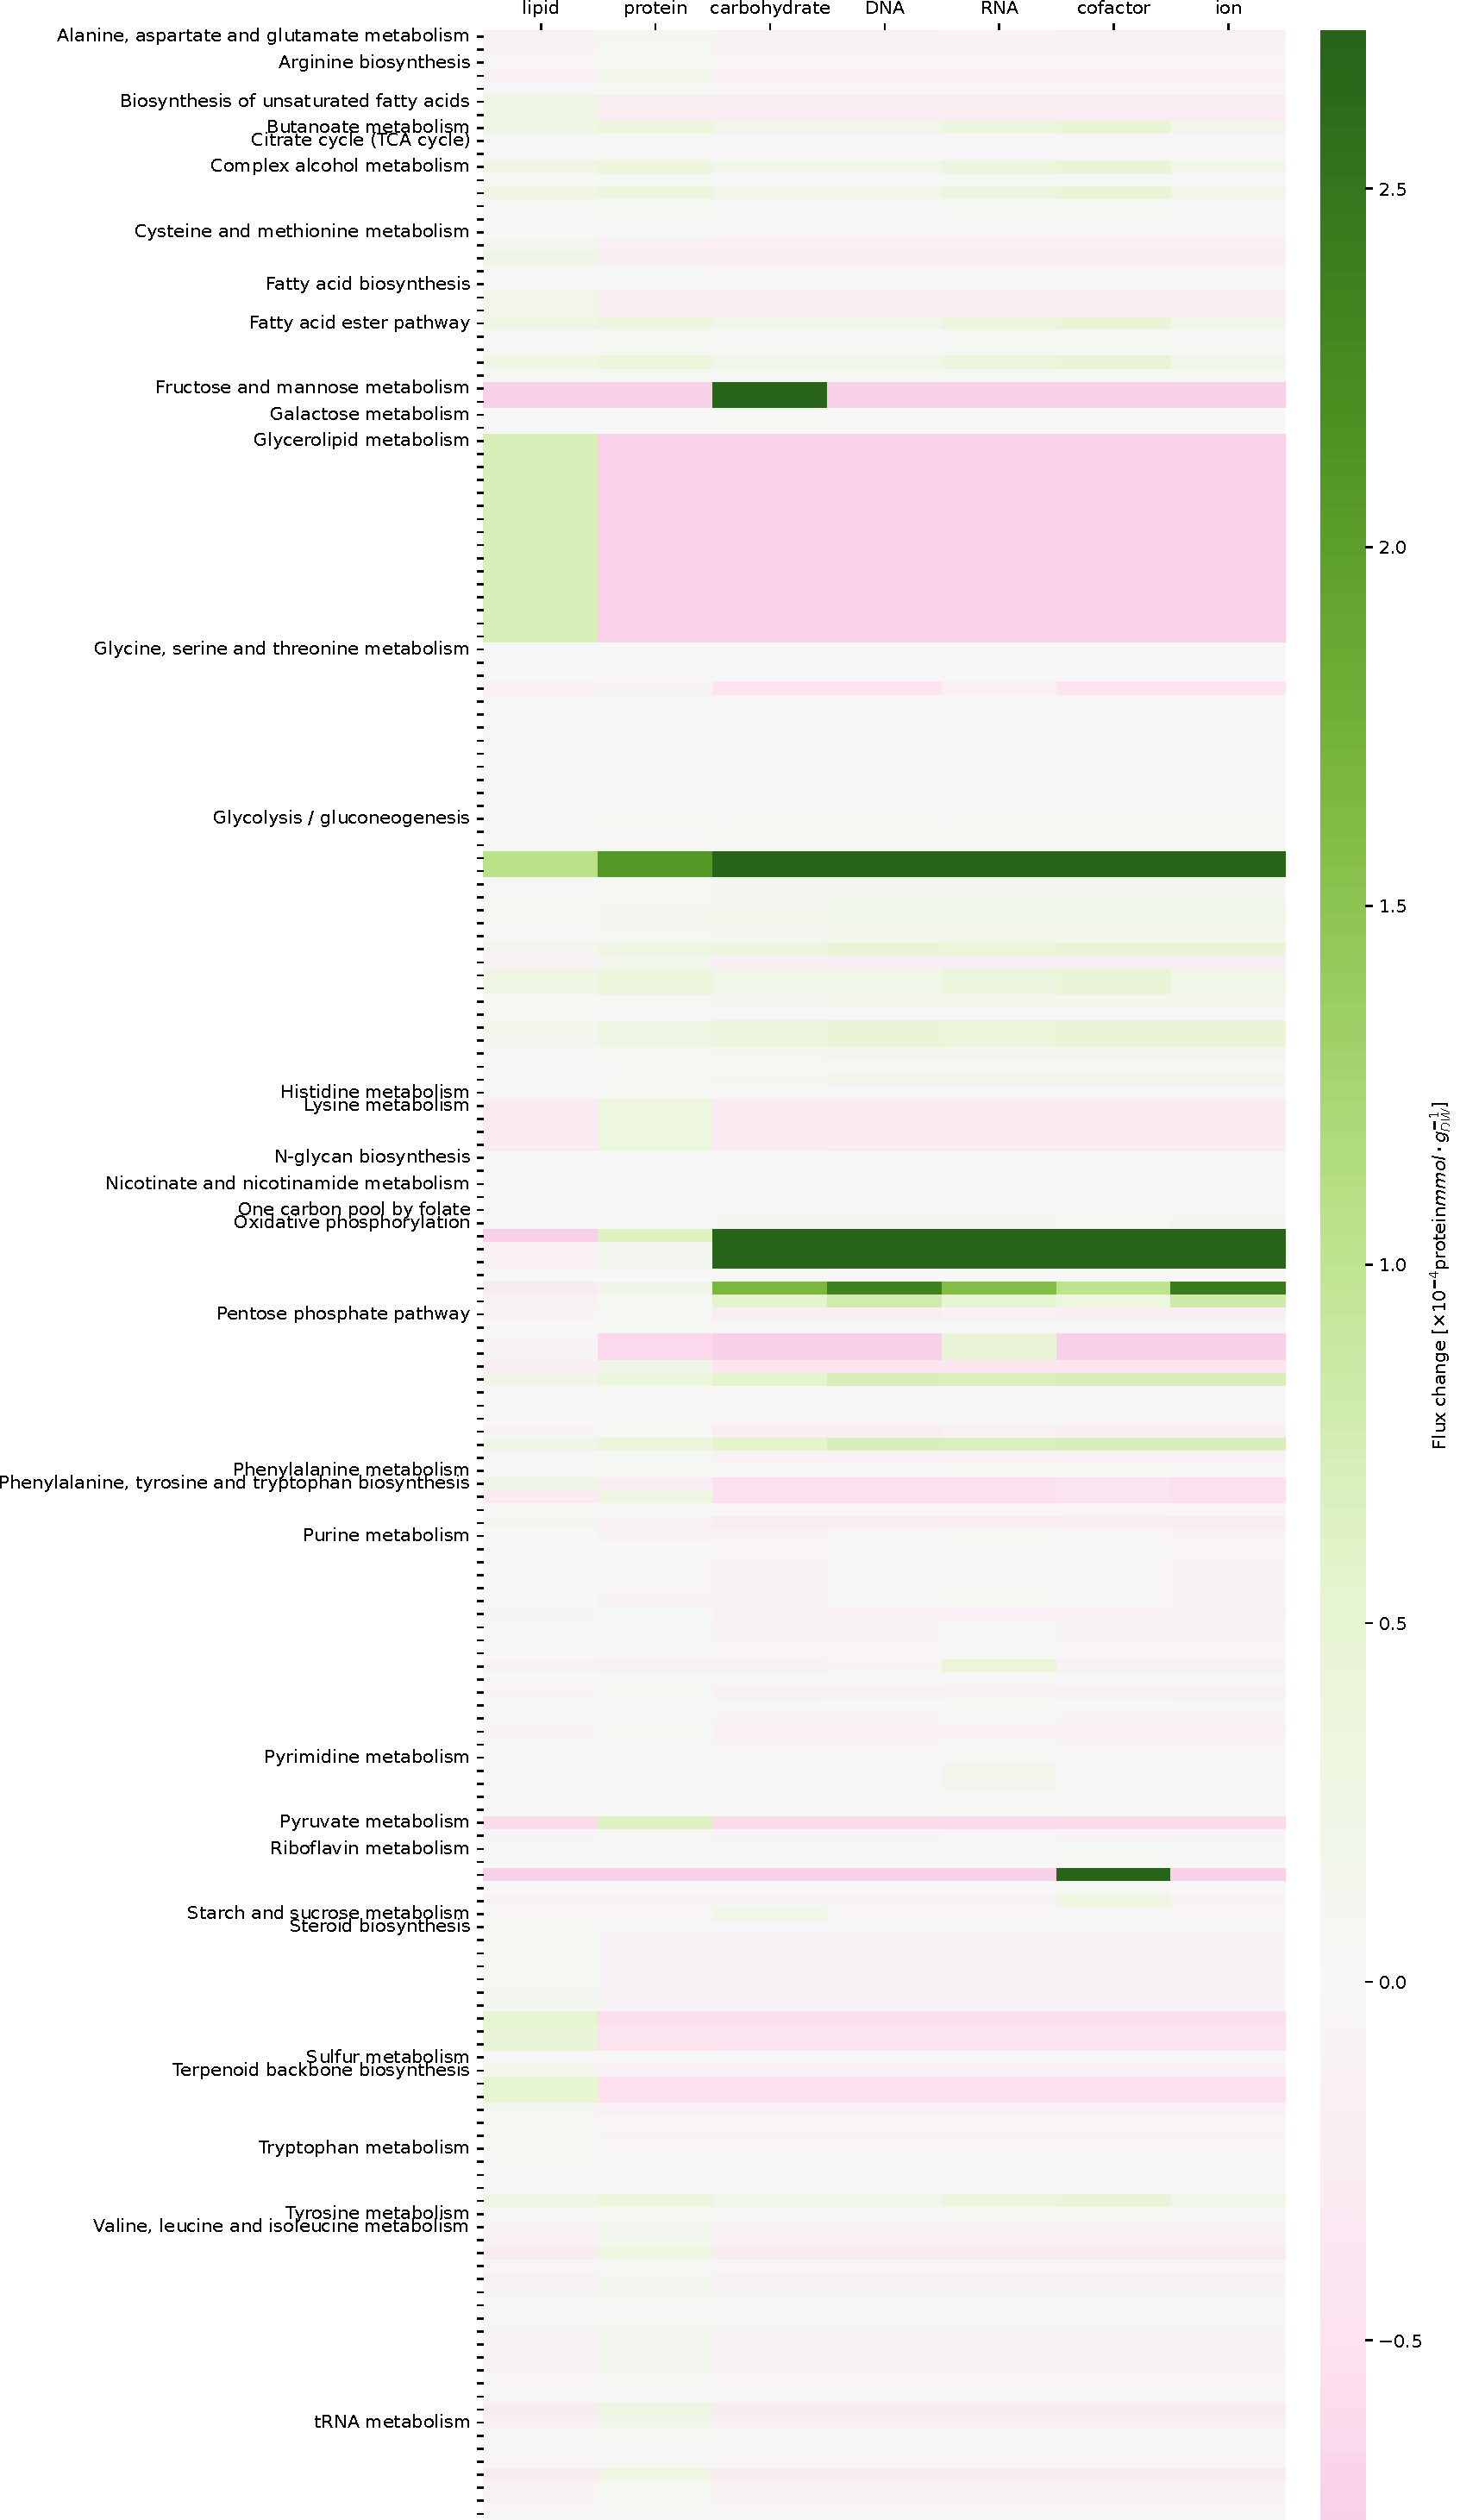
\includegraphics[width=.8\linewidth]{abl_vs_enz_use_plots_adapted}
  \caption{
    The cell changes how it allocates its proteome to enzymes when different components of its biomass are prioritised.
    Each column shows the component that remains in each round of pseudometabolite ablation.
    Rows represent reactions, sorted by subsystem.
    Colours represent how the cell re-allocates its proteome to each enzyme: green shows an increase in enzyme usage reaction ($ER_{i}$,~equation \ref{eq:model-gecko-enzyme-usage}) flux, representing more of the proteome allocated to the production of the relevant enzyme, while pink shows a decrease in flux, representing less of the proteome allocated to the enzyme.
    Flux changes with magnitudes smaller than \SI{3d-6}{\milli\mole~\gram_{DW}^{-1}} are excluded to restrict the number of enzymes, of which there are more than \num{4000}, to aid display purposes.
  }
  \label{fig:model-ablate-enz-use}
\end{figure}

Investigate proteome allocation as sanity check (figure~\ref{fig:model-ablate-enz-use}):

\begin{enumerate}
  \item Increased fatty acid biosynthesis, fatty acid ester pathway, glycerolipid metabolism, steroid biosynthesis, terpenoid backbone biosynthesis when lipid is prioritised.
        Decreased oxidative phosphorylation.
  \item Small increases in amino acid metabolism and oxidative phosphorylation when protein is prioritised.
        Pyruvate metabolism increases too.
  \item Strong increase in fructose and mannose metabolism when carbohydrate is prioritised.
        Strong increase in riboflavin metabolism when cofactor is prioritised (riboflavin is a cofactor).
        Increase in pentose phosphate pathway, purine metabolism, and pyrimidine metabolism when RNA is prioritised.
        However, decrease in pentose phosphate pathway when DNA is prioritised.
  \item For carbohydrate, DNA, RNA, cofactor, ion, strong increases in glycolysis/gluconeogenesis and oxidative phosphorylation.
  \item Main conclusion is enzyme usage flux changes are as expected.
\end{enumerate}

\section{Estimating timescale of biosynthesis}
\label{sec:model-timescale}

I used the ecYeast8.6.0 model with glucose uptake restricted to within [0, 16.89]
This number is based on the glucose uptake rate from using the non-modified model to optimise growth rate.
This value agrees with theoretical saturation rates of 16--19 \SI{}{\milli\mol~\gram_{DW}^{-1}} \parencite{blankTCACycleActivity2004}.
Using the biomass reaction as the objective function, I optimise the model to obtain the predicted growth rate, and computed the doubling time based on this growth rate as follows:

\begin{equation}
  t = \frac{\ln 2}{\lambda}
  \label{eq:model-doubling-time}
\end{equation}

where $t$ is the doubling time and $\lambda$ is the growth rate, equivalent to the optimal flux of the biomass reaction.

I ablate components in biomass reaction that have pseudoreactions associated with the `Growth' subsystem, as discussed in section~\ref{sec:model-yeast8-pseudometabolites} in turn.
In each round, the model is simulated, using the modified biomass reaction as the objective function, and the flux is recorded.
Doubling time is computed, taking into account the mass fraction of each biomass component -- i.e.\ if the component is a smaller fraction of the cell, it takes less time.
Specifically, the computation is:

\begin{equation}
  t_{i}^{\prime} = f_{i} \cdot \frac{\ln 2}{\lambda_{i}^{\prime}}
  \label{eq:model-ablated-time}
\end{equation}

where $i$ represents each of the biomass components (lipids, proteins, carbohydrates, DNA, RNA, cofactors, and ions), $t_{i}$ is the predicted time for synthesis of each biomass component, $f_{i}$ is the mass fraction of each biomass component, and $\lambda_{i}^{\prime}$ is optimal flux of the ablated biomass reaction.
$f_{i}$ for each biomass component is computed by dividing the molecular weight of the corresponding pseudometabolite by the molecular weight of biomass (table~\ref{tab:ecyeast8-mol-weights}).

For comparison, I computed estimates of the time for each biomass component, assuming that it is proportional to the mass fraction:

\begin{equation}
  t_{i} = f_{i} \cdot t
  \label{eq:model-proportional-time}
\end{equation}

where $t$ is the doubling time found in equation~\ref{eq:model-doubling-time}.

\begin{figure}
  \centering
  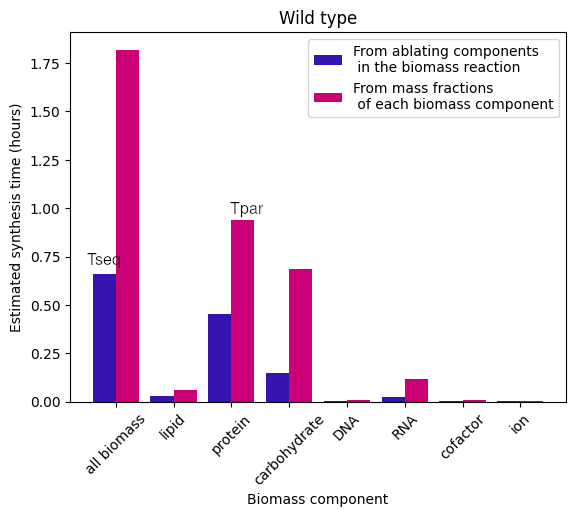
\includegraphics[width=.9\linewidth]{ablation_example_ratio.png}
  \caption{
    Comparing time scales derived from ablating components of the biomass reaction (blue) and from assuming that synthesis time is proportional to the mass fraction of the biomass component (red).
    Times for each biomass component (lipid, protein, carbohydrate, DNA, RNA, cofactor, ion) were computed according to equations~\ref{eq:model-ablated-time}--\ref{eq:model-proportional-time}.
    Blue under `all biomass' is the sum of times derived from ablation (other blue bars), while red under `all biomass' is derived from the flux of the original biomass reaction (equation~\ref{eq:model-doubling-time}).
    As a summary value, the ratio between the total time predicted by ablation and the biomass component that is predicted to take the most time is computed (ratio = A/B, as on figure).
  }
  \label{fig:model-ablate-times}
\end{figure}

And as a summary value, the ratio between the total time predicted by ablation and the biomass component that is predicted to take the most time is computed (ratio = A/B, as on figure).
A represents sum of times from focusing on each biomass component -- thus representing time predicted, assuming biomass components are synthesised in turn:

\begin{equation}
  A = \sum_{i} t_{i}^{\prime} = \sum f_{i} \cdot \frac{\ln 2}{\lambda_{i}^{\prime}}
  \label{eq:model-a}
\end{equation}

B represents greatest time of synthesis of the biomass component if time is assumed to be proportional to mass fraction.
This is always protein as it accounts for $\approx$50\% of the mass fraction:

\begin{equation}
  B = \argmax_{i} t_{i} = t_{\mathrm{protein}} = f_{\mathrm{protein}} \cdot \frac{\ln 2}{\lambda_{0}}; \because \argmax_{i} f_{i} = f_{\mathrm{protein}}
  \label{eq:model-b}
\end{equation}

B thus represents the limiting, slowest process.

Therefore,

\begin{equation}
  r = \frac{A}{B} = (\sum_i \frac{f_i}{\lambda_i^\prime}) \cdot \frac{\lambda_0}{f_{\mathrm{protein}}} = (\frac{f_{\mathrm{lipid}}}{\lambda_{\mathrm{lipid}}^\prime} + \frac{f_{\mathrm{protein}}}{\lambda_{\mathrm{protein}}^\prime} + \ldots + \frac{f_{\mathrm{ion}}}{\lambda_{\mathrm{ion}}^\prime}) \cdot \frac{\lambda_0}{f_{\mathrm{protein}}}
  \label{eq:model-ratio}
\end{equation}

This expression means that the definition of the $r$ ratio is not trivial and depends on the $\lambda_{0}$ and the $\lambda_{i}^{\prime}$ values, which are all independent of each other.

A smaller A/B ratio (< 1) means that --- under these conditions --- synthesising biomass components in sequence saves more time.
In figure~\ref{fig:model-ablate-times}, the ratio is 0.70.

The fact that this still holds true for auxotrophs and deletion strains supports experimental evidence that auxotrophs and deletion strains have YMCs (figure~\ref{fig:model-ablation-strains}).

\begin{figure}
  \centering
  \begin{subfigure}[htpb]{0.45\textwidth}
   \centering
   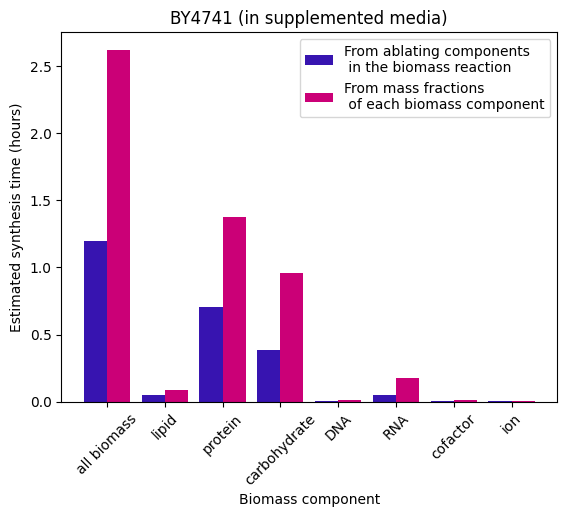
\includegraphics[width=\textwidth]{ablation_by4741}
   \caption{
     BY4741
   }
   \label{fig:model-ablation-by4741}
  \end{subfigure}
  \begin{subfigure}[htpb]{0.45\textwidth}
   \centering
   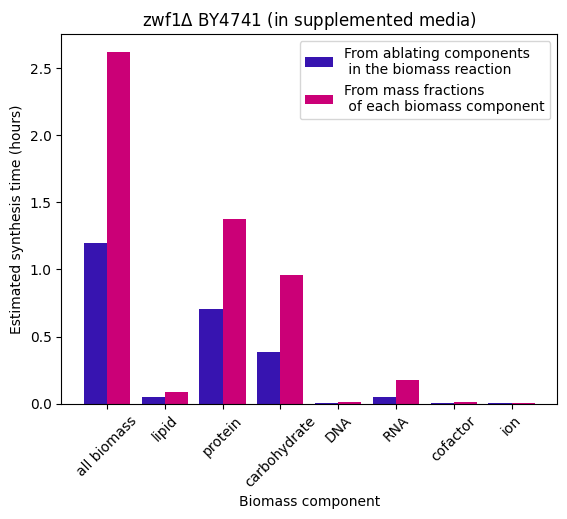
\includegraphics[width=\textwidth]{ablation_zwf1}
   \caption{
     zwf$\Delta$ in the BY4741 background.
   }
   \label{fig:model-ablation-zwf1}
  \end{subfigure}
  \begin{subfigure}[htpb]{0.45\textwidth}
   \centering
   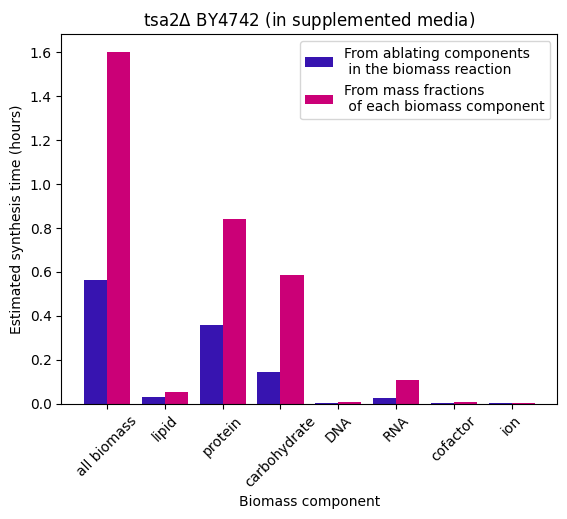
\includegraphics[width=\textwidth]{ablation_tsa2}
   \caption{
     tsa2$\Delta$ in the BY4742 background.  The ecYeast8 model does not include reactions that correspond to \textit{TSA1}.
   }
   \label{fig:model-ablation-tsa2}
  \end{subfigure}
  \caption{
    Ablation barplots of auxotrophs and deletion strains.
    For BY4741-background strains, supplements are simulated by allowing uptake of histidine, leucine, tryptophan, methionine and uracil.
    The same applied to BY4742-background strains, but lysine uptake replaces methionine uptake.
  }
  \label{fig:model-ablation-strains}
\end{figure}
% Adding supplements, e.g. amino acids, dNTPs/NTPs, pyruvate, glucose limitation?
% Or do C/N grid heatmaps demonstrate this.

\section{Effect of restricting the enzyme pool}
\label{sec:model-pool}

\begin{figure}
  \centering
  \begin{subfigure}[htpb]{0.45\textwidth}
   \centering
   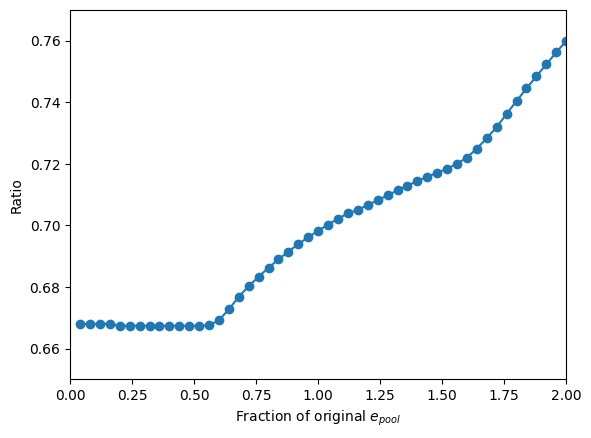
\includegraphics[width=\textwidth]{epool_ec_ratio_shrinkyaxis}
   \caption{
     Effect on ratio ($r$).
   }
   \label{fig:model-pool-ratio}
  \end{subfigure}
  \begin{subfigure}[htpb]{0.45\textwidth}
   \centering
   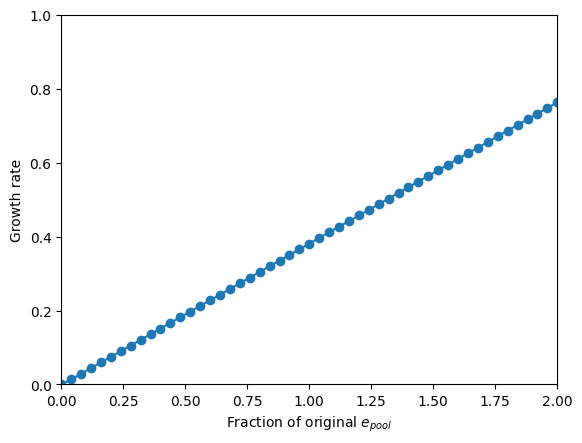
\includegraphics[width=\textwidth]{epool_ec_gr}
   \caption{
     Effect on wild type growth rate ($\lambda_{0}$).
   }
   \label{fig:model-pool-growthrate}
  \end{subfigure}
  \begin{subfigure}[htpb]{0.45\textwidth}
   \centering
   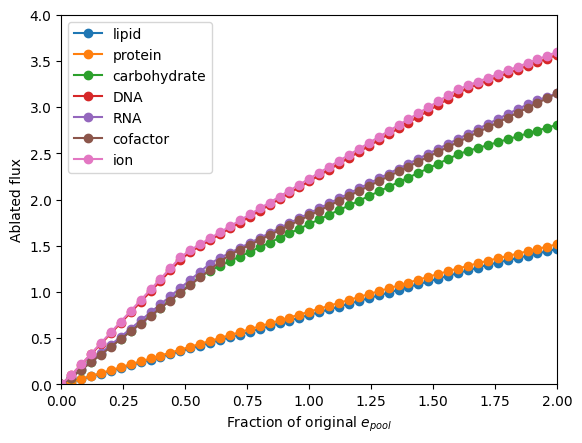
\includegraphics[width=\textwidth]{epool_ec_components}
   \caption{
     Effect on ablated growth rates ($\lambda_{i}^{\prime}$).
   }
   \label{fig:model-pool-ablated}
  \end{subfigure}
  \caption{
    Constraining the proteome pool available for synthesis enzymes (decreasing $e_{\mathrm{pool}}$) leads to a greater advantage of sequential biosynthesis of biomass components over parallel biosynthesis, as evidenced by a decreasing $r$ ratio (\ref{fig:model-pool-ratio}).
    Concurrently, the wild type growth rate ($\lambda_{0}$) decreases linearly to zero (\ref{fig:model-pool-growthrate}) and ablated growth rates ($\lambda_{i}^{\prime}$) decrease in linear segments independently of each other and of the growth rate (\ref{fig:model-pool-growthrate}); these values determine the ratio according to equation~\ref{eq:model-ratio}.
  }
  \label{fig:model-pool}
\end{figure}


Interpretation of figure~\ref{fig:model-pool}...

\begin{itemize}
  \item Decide on restricting $e_{\mathrm{pool}} \in [0, 2]$ to give realistic growth rates.
  \item Growth rate varies linearly as $e_{\mathrm{pool}}$ varies.
  \item However, the ratio is not constant, but climbs up in steps --- derivation to follow.
        With higher $e_{\mathrm{pool}}$ values (less of a constraint on the enzyme pool), the ratio increases, indicating less advantage for sequential biosynthesis.
        Here, ratio < 1, but we've seen ratios > 1 in certain nutrient conditions (fig~\ref{fig:model-grid-glc},~\ref{fig:model-grid-pyr}).
  \item As $e_{\mathrm{pool}}$ increases, ablated flux all start out linear/linear-ish.
        But then the gradient of these lines change at various points, all going to a plateau at very high $e_{\mathrm{pool}}$ (not shown here).
  \item Ablated flux doesn't always vary linearly as $e_{\mathrm{pool}}$ varies --- only protein and lipid are linear in this region
        Perhaps this means that $e_{\mathrm{pool}}$ is limiting for these (expensive) components, and less so the case for the others.
  \item This also confirms that ablated flux traces don't always have to increase linearly and are independent of the growth rate traces.
\end{itemize}

TODO: add differential calculus to show that the plots make sense mathematically.

Other methods considered to minimise protein cost:
\begin{itemize}
  \item Parsimonious FBA \parencite{lewisOmicDataEvolved2010}.
    \begin{itemize}
      \item This first uses FBA to compute optimal growth rate, fixes this value, then minimises sum of gene-associated reaction fluxes while maintaining optimal growth (either minimises the sum of fluxes or squared sum, depending on the software package).
      \item Rejected because it fixes the growth rate, but we want to see how constraints affect cell strategies as they vary along a spectrum.
        And also because it relies on reducing the subset of genes that contribute to the solution --- it modifies the model and it also relies on good gene-protein annotations.
    \end{itemize}
  \item Regularised FBA.
    \begin{itemize}
      \item \textcite{vijayakumarHybridFluxBalance2020} describe a quadratic program for solving a regularised bi-level FBA, i.e.\: $\max g^\intercal v - \frac{\sigma}{2}v^\intercal v$ where $g$ is the objective function, $v$ is the flux vector, and $\sigma$ is a regularisation parameter than can be tuned.
      \item Rejected because it requires a quadratic solver, thus difficult and computationally expensive to implement.
            And because the behaviour is not as expected, i.e.\ the growth rate does not change as the regularisation parameter $\sigma$ varies, even though we expected a trade-off between growth and reaction fluxes to change as this parameter varies.
    \end{itemize}
  \item Constrain the sum of absolute values of fluxes.
    \begin{itemize}
      \item Namely, $\sum |v| < c$, where $c$ is a constant to be varied.
      \item This makes sense for the Yeast8 (no enzyme constraint) model, and as $c$ decreases to 0, the original growth rate $\lambda_{0}$ and ablated growth rates $\lambda_{i}^{\prime}$ decreased to 0 linearly, while the $r$ ratio remains constant.
            ADD PLOTS TO SHOW THIS?
    \end{itemize}
\end{itemize}

The last method, if if applied to ecYeast8,
there is potential double-/triple-counting of imposing constraints, i.e.\:
\begin{enumerate}
  \item constraints on enzyme usage imposed on the enzyme-usage pseudoreactions created by GECKO,
  \item constraints on sum of the absolute values of fluxes.
\end{enumerate}
This will confuse interpretation.

Therefore, I decide to vary $e_{\mathrm{pool}}$ to study proteomic constraints as this takes advantage of a formalism that already exists in ecYeast8, by virtue of GECKO, that is easy to interpret and modify.


\section{Effect of carbon and nitrogen sources}
\label{sec:model-exchange}

\subsection{Exchange reaction saturation}
\label{subsec:model-saturation}

FBA models include nutrient exchange reactions to simulate the presence of certain nutrients in the growth medium.
Because FBA models do not account for substrate concentrations, studying the effect of nutrient sources in FBA models involves constraining the flux of such exchange reactions to achieve validated growth rates, as performed by \textcite{elsemmanWholecellModelingYeast2022} to study the effect of glucose.

Using the ecYeast8.6.0 model, I varied the flux bounds of exchange reaction and recorded how it affects predicted growth rate.
I did this with two carbon sources, glucose and pyruvate, and with ammonium as a nitrogen source (figure~\ref{fig:model-saturation}).

\begin{figure}
  \centering
  \begin{subfigure}[t]{0.45\textwidth}
  \centering
    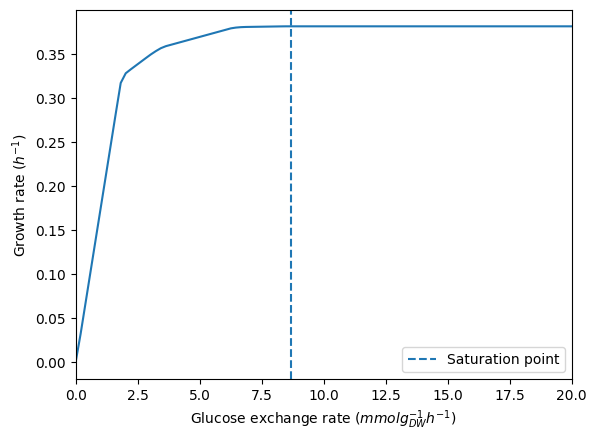
\includegraphics[width=\linewidth]{saturation_glc}
    \caption{
      Effect of glucose exchange on growth rate.
      Growth rate saturation is at \SI{8.69}{\milli\mole~\gram_{DW}^{-1}~\hour^{-1}}.
    }
    \label{fig:model-saturation-glucose}
  \end{subfigure}%
  \begin{subfigure}[t]{0.45\textwidth}
  \centering
    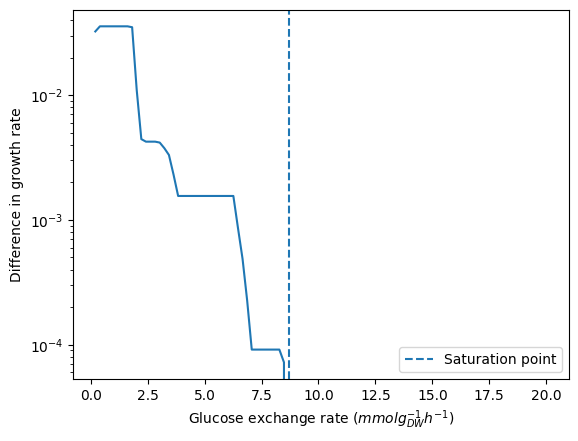
\includegraphics[width=\linewidth]{saturation_diff_glc}
    \caption{
    }
    \label{fig:model-saturation-diff-glucose}
  \end{subfigure}

  \begin{subfigure}[t]{0.45\textwidth}
  \centering
    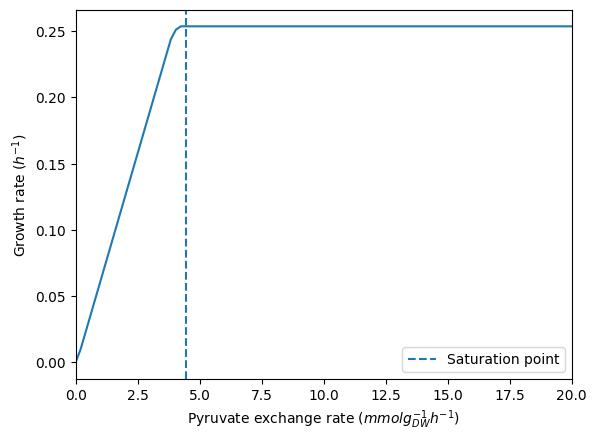
\includegraphics[width=\linewidth]{saturation_pyr}
    \caption{
      Effect of pyruvate exchange on growth rate.
      Growth rate saturation is at \SI{4.44}{\milli\mole~\gram_{DW}^{-1}~\hour^{-1}}.
    }
    \label{fig:model-saturation-pyruvate}
  \end{subfigure}%
  \begin{subfigure}[t]{0.45\textwidth}
  \centering
    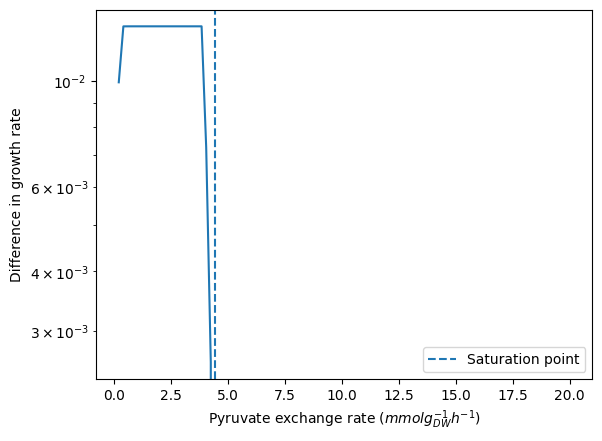
\includegraphics[width=\linewidth]{saturation_diff_pyr}
    \caption{
    }
    \label{fig:model-saturation-diff-pyruvate}
  \end{subfigure}

  \begin{subfigure}[t]{0.45\textwidth}
  \centering
    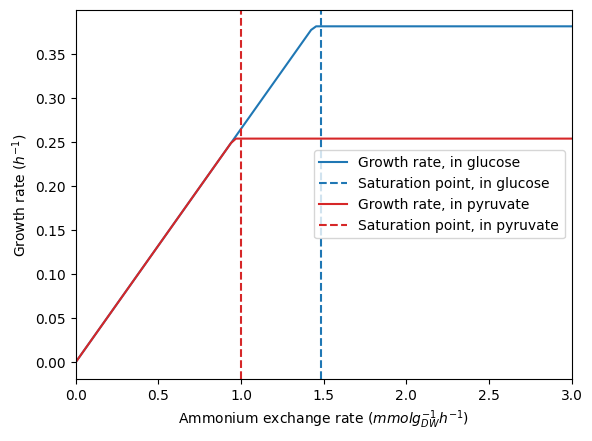
\includegraphics[width=\linewidth]{saturation_amm}
    \caption{
      Effect of ammonium exchange on growth rate, with exchanges of carbon sources set to growth rate saturation based on figures~\ref{fig:model-saturation-glucose} and ~\ref{fig:model-saturation-pyruvate}.
      Growth rate saturation is at \SI{1.48}{\milli\mole~\gram_{DW}^{-1}~\hour^{-1}} in glucose, and
      at \SI{1.00}{\milli\mole~\gram_{DW}^{-1}~\hour^{-1}} in pyruvate.
    }
    \label{fig:model-saturation-ammonium}
  \end{subfigure}%
  \begin{subfigure}[t]{0.45\textwidth}
  \centering
    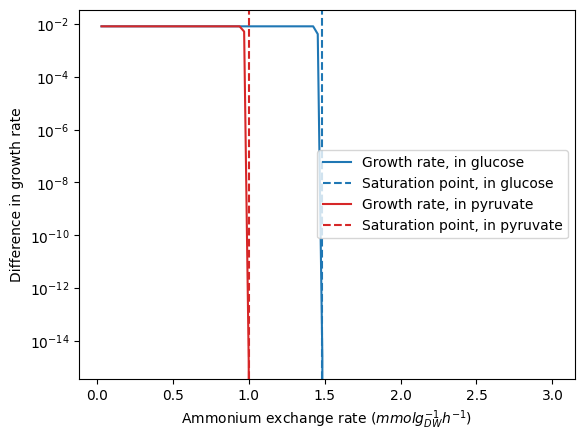
\includegraphics[width=\linewidth]{saturation_diff_amm}
    \caption{
    }
    \label{fig:model-saturation-diff-ammonium}
  \end{subfigure}

  \caption{
    Effect of nutrient exchange reactions on growth rate, predicted by the ecYeast8 model (left panels).
    To demonstrate how saturation values were found,
    right panels (\ref{fig:model-saturation-diff-glucose},~\ref{fig:model-saturation-diff-pyruvate},~\ref{fig:model-saturation-diff-ammonium}) show discrete differences of growth rates with respect to exchange rates.
  }
  \label{fig:model-saturation}
\end{figure}

This shows:
\begin{itemize}
  \item The glucose saturation curve is similar to that predicted by \textcite{elsemmanWholecellModelingYeast2022} using another derivative of the Yeast8 model.
        The saturation point is well below the maximal glucose consumption rate of \SIrange{16}{19}{\milli\mole~\gram_{DW}^{-1}~\hour^{-1}} as determined by GC-MS-based metabolic flux ratio analysis \parencite{blankTCACycleActivity2004}.
  \item The maximum growth rate on glucose is \SI{0.38}{\hour^{-1}} while the maximum growth rate on pyruvate is \SI{0.25}{\hour^{-1}}.
        The glucose value agrees with \textcite{domenzainReconstructionCatalogueGenomescale2022}, which uses latest published version of GECKO to create the ecYeast7 model to predict maximum growth rates on various carbon sources, and also agrees with my experimental observations.
        This study did not predict growth rate on pyruvate, but a lower maximum growth rate on a non-fermentable carbon source compared to glucose agrees with the biochemical basis and is also consistent with my experimental observations.
  \item The growth rate saturation point for ammonium is determined by the maximal growth rate determined by each carbon source.
\end{itemize}

\subsection{Effect of carbon and nitrogen sources on biomass synthesis strategies}
\label{subsec:model-grid}

\begin{figure}
  \centering
  \begin{subfigure}[t]{0.45\textwidth}
  \centering
    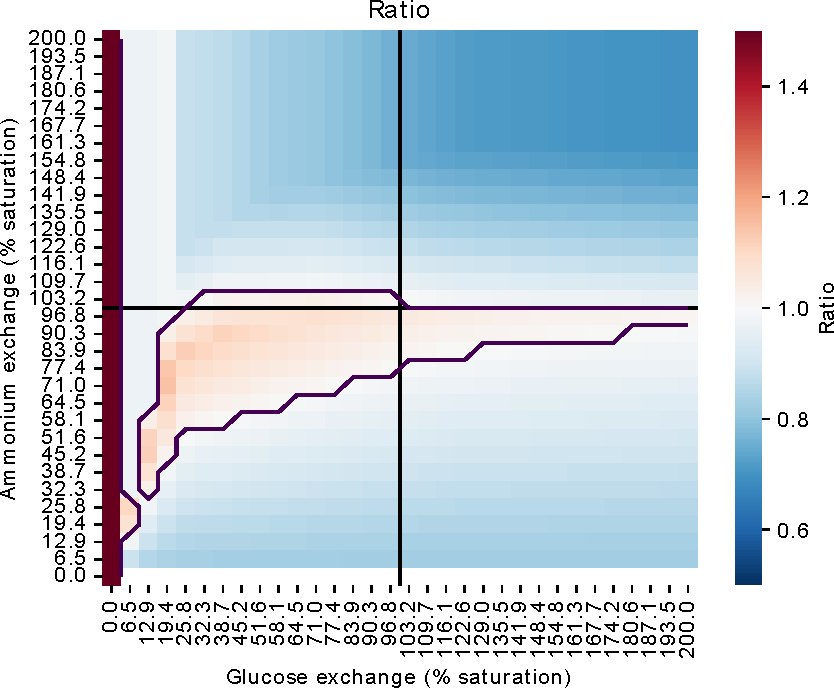
\includegraphics[width=\linewidth]{ec_grid_glc_amm_ratio}
    \caption{
      Ratio ($r$)
    }
    \label{fig:model-grid-glc-ratio}
  \end{subfigure}%
  \begin{subfigure}[t]{0.45\textwidth}
  \centering
    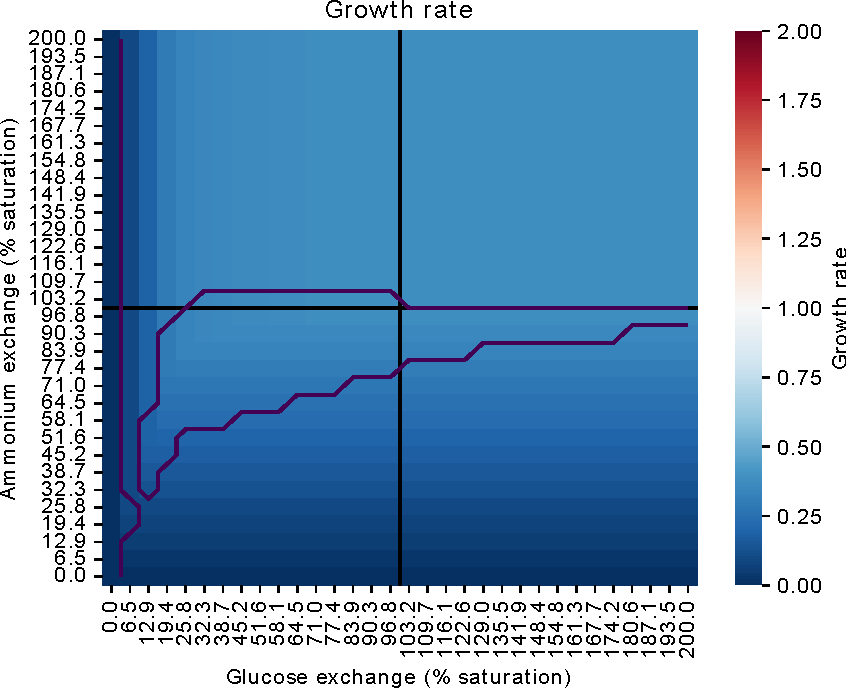
\includegraphics[width=\linewidth]{ec_grid_glc_amm_growthrate}
    \caption{
      Growth rate based on unmodified biomass reaction ($\lambda_{0}$)
    }
    \label{fig:model-grid-glc-growthrate}
  \end{subfigure}

  \begin{subfigure}[t]{0.45\textwidth}
  \centering
    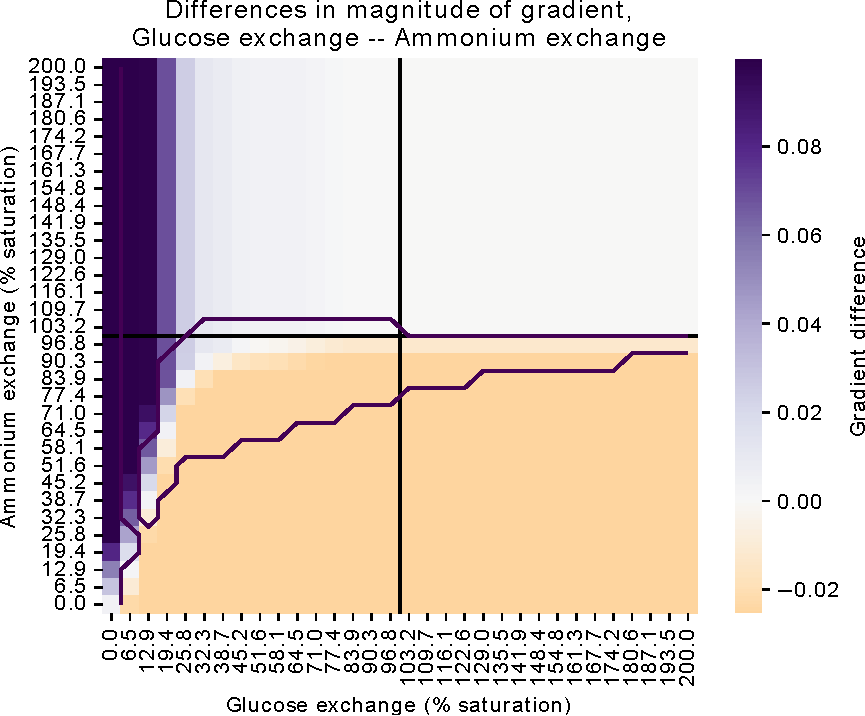
\includegraphics[width=\linewidth]{ec_grid_glc_amm_gradient_compare}
    \caption{
      Differences in magnitude of gradients across axes ($|\frac{\Delta \lambda_{0}}{\Delta R_{\mathrm{glucose}}}| - |\frac{\Delta \lambda_{0}}{\Delta R_{\mathrm{ammonium}}}|$).
      %Positive values (indigo) indicate glucose-limiting conditions, while negative values (beige) indicate ammonium-limiting conditions.
    }
    \label{fig:model-grid-glc-gradient-compare}
  \end{subfigure}%
  \begin{subfigure}[t]{0.45\textwidth}
  \centering
    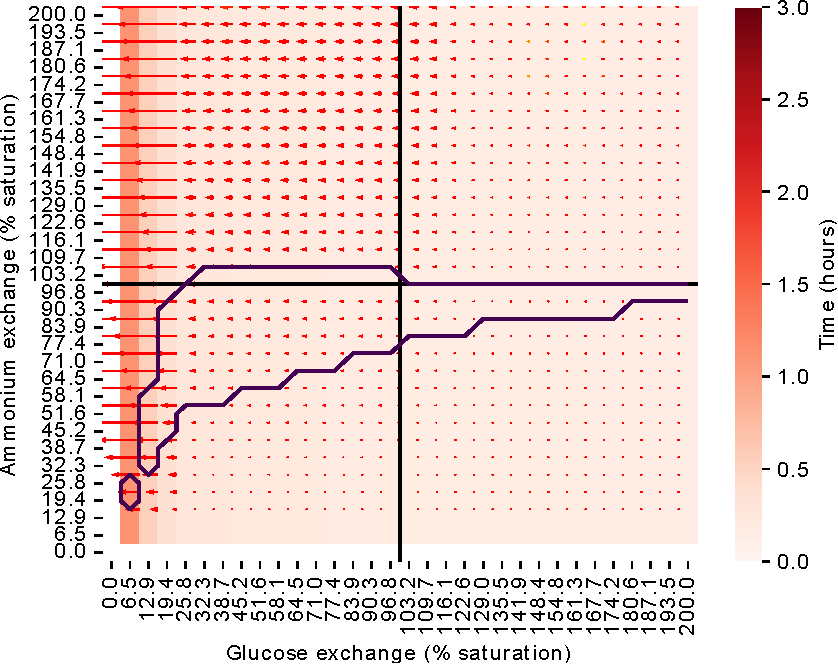
\includegraphics[width=\linewidth]{ec_grid_glc_amm_carb}
    \caption{
      $t_{\mathrm{carbohydrate}}^{\prime}$
    }
    \label{fig:model-grid-glc-carb}
  \end{subfigure}

  \begin{subfigure}[t]{0.45\textwidth}
  \centering
    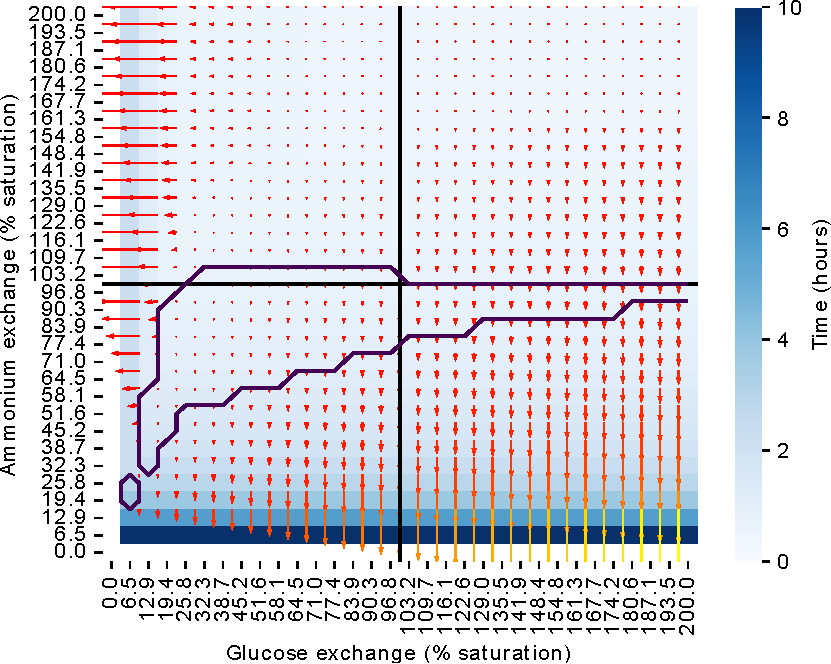
\includegraphics[width=\linewidth]{ec_grid_glc_amm_prot}
    \caption{
      $t_{\mathrm{protein}}^{\prime}$
    }
    \label{fig:model-grid-glc-prot}
  \end{subfigure}%
  \begin{subfigure}[t]{0.45\textwidth}
  \centering
    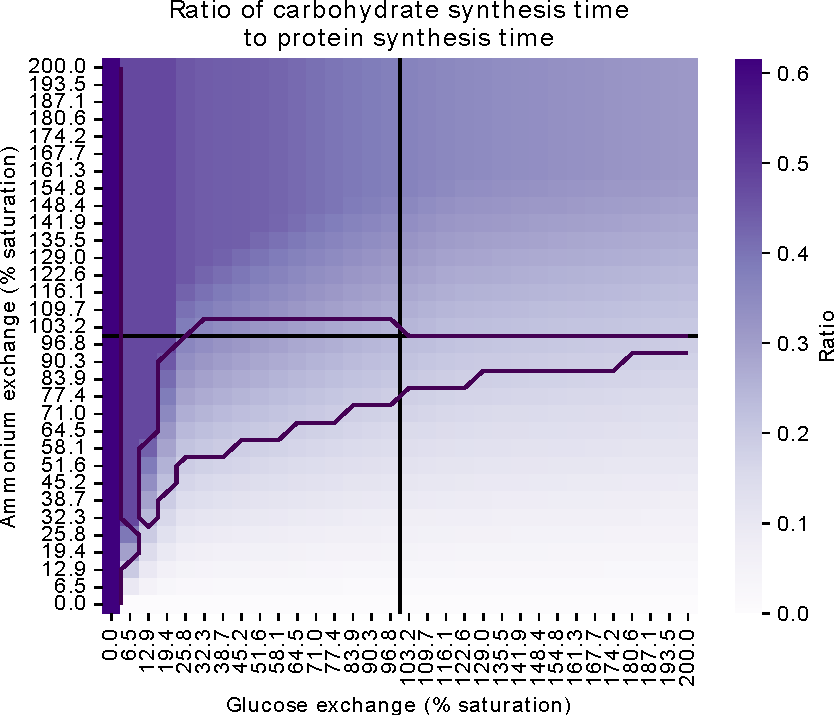
\includegraphics[width=\linewidth]{ec_grid_glc_amm_carb_to_prot}
    \caption{
      $t_{\mathrm{carbohydrate}}^{\prime}/t_{\mathrm{protein}}^{\prime}$
    }
    \label{fig:model-grid-glc-carb-to-prot}
  \end{subfigure}
  \caption{
    Effect of glucose ($R_{\mathrm{glucose}}$) and ammonium exchange rates ($R_{{\mathrm{ammonium}}}$) on various quantities.
    Exchange rates are expressed in percentages of growth saturation values shown in~\ref{fig:model-saturation}: glucose saturation being at \SI{8.69}{\milli\mole~\gram_{DW}^{-1}~\hour^{-1}} and ammonium saturation being at \SI{1.48}{\milli\mole~\gram_{DW}^{-1}~\hour^{-1}}.
    Black straight lines indicate saturation values.
    Contours show region in which ratio $r > 1$.
  }
  \label{fig:model-grid-glc}
\end{figure}

\begin{figure}
  \centering
  \begin{subfigure}[t]{0.45\textwidth}
  \centering
    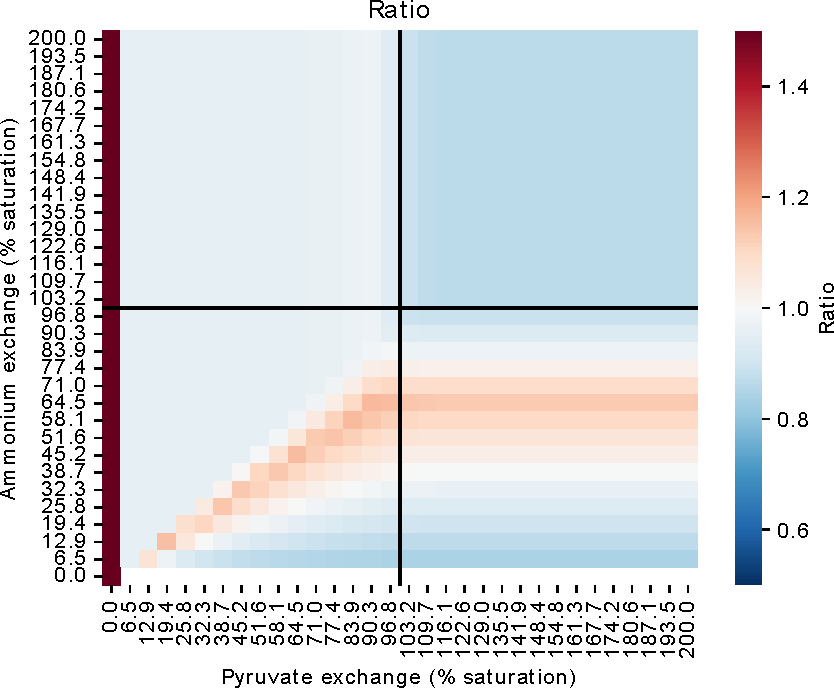
\includegraphics[width=\linewidth]{ec_grid_pyr_amm_ratio}
    \caption{
      Ratio ($r$)
    }
    \label{fig:model-grid-pyr-ratio}
  \end{subfigure}%
  \begin{subfigure}[t]{0.45\textwidth}
  \centering
    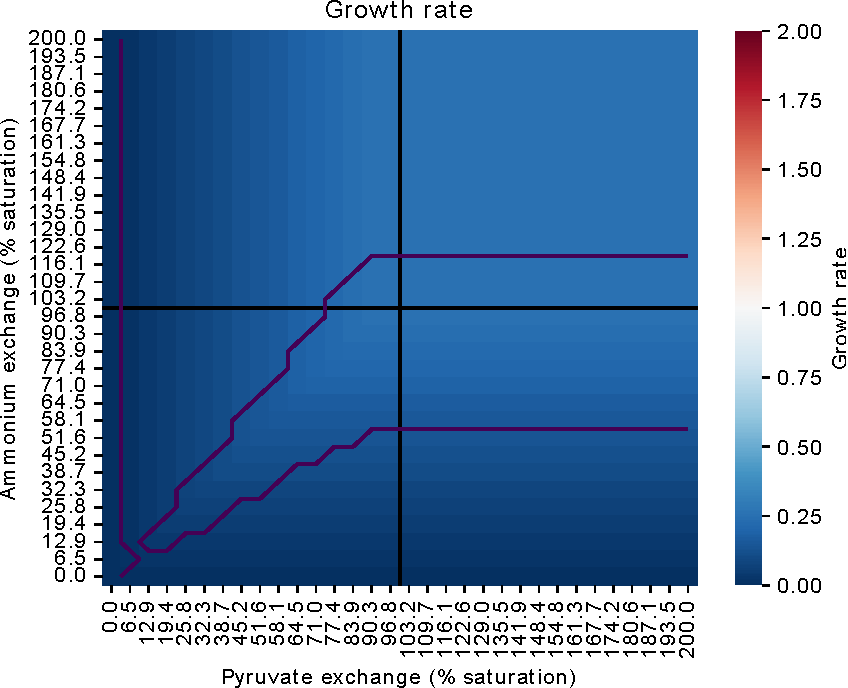
\includegraphics[width=\linewidth]{ec_grid_pyr_amm_growthrate}
    \caption{
      Growth rate based on unmodified biomass reaction ($\lambda_{0}$)
    }
    \label{fig:model-grid-pyr-growthrate}
  \end{subfigure}

  \begin{subfigure}[t]{0.45\textwidth}
  \centering
    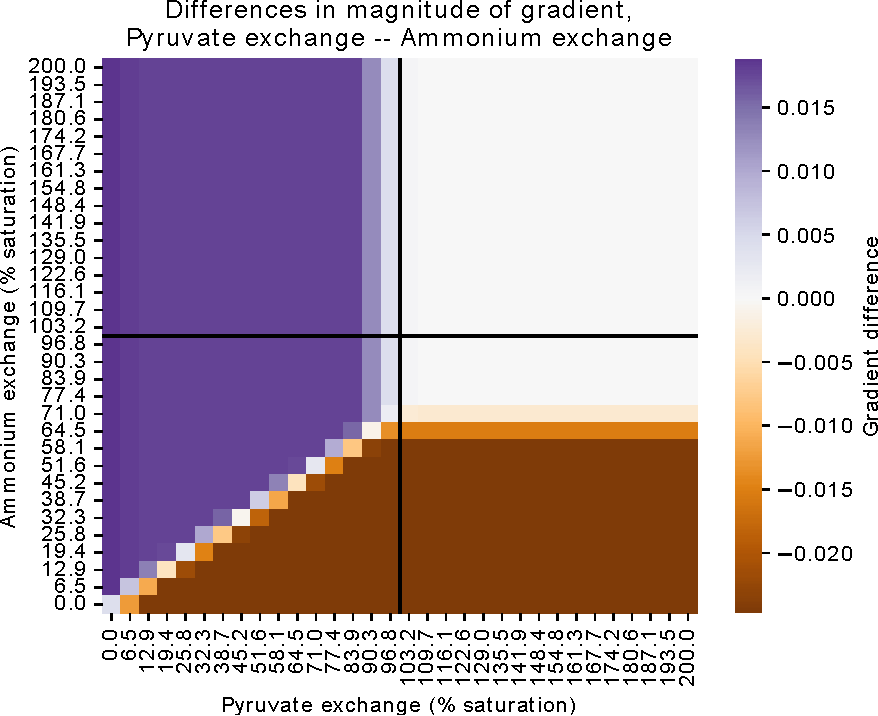
\includegraphics[width=\linewidth]{ec_grid_pyr_amm_gradient_compare}
    \caption{
      Differences in magnitude of gradients across axes ($|\frac{\Delta \lambda_{0}}{\Delta R_{\mathrm{pyruvate}}}| - |\frac{\Delta \lambda_{0}}{\Delta R_{\mathrm{ammonium}}}|$).
    }
    \label{fig:model-grid-pyr-gradient-compare}
  \end{subfigure}%
  \begin{subfigure}[t]{0.45\textwidth}
  \centering
    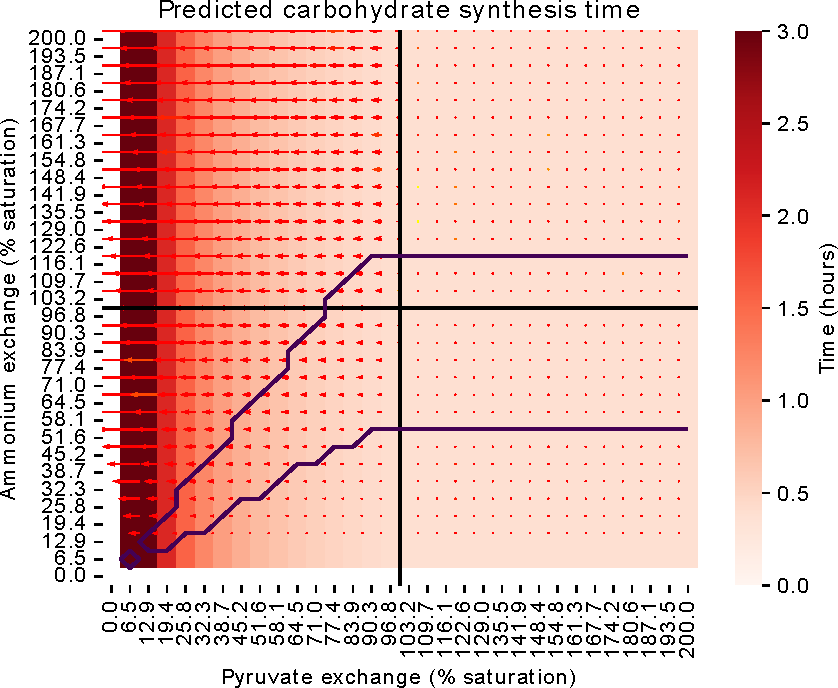
\includegraphics[width=\linewidth]{ec_grid_pyr_amm_carb}
    \caption{
      $t_{\mathrm{carbohydrate}}^{\prime}$
    }
    \label{fig:model-grid-pyr-carb}
  \end{subfigure}

  \begin{subfigure}[t]{0.45\textwidth}
  \centering
    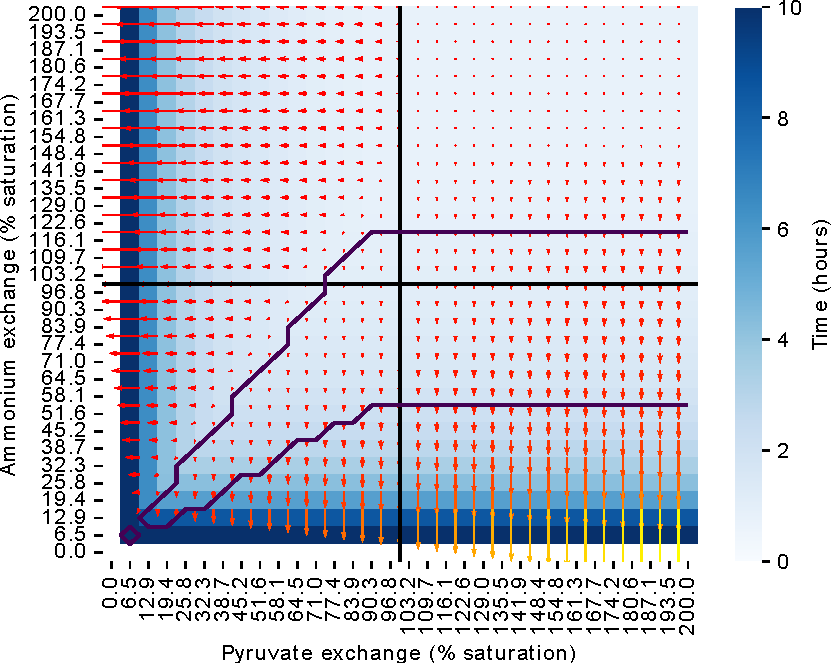
\includegraphics[width=\linewidth]{ec_grid_pyr_amm_prot}
    \caption{
      $t_{\mathrm{protein}}^{\prime}$
    }
    \label{fig:model-grid-pyr-prot}
  \end{subfigure}%
  \begin{subfigure}[t]{0.45\textwidth}
  \centering
    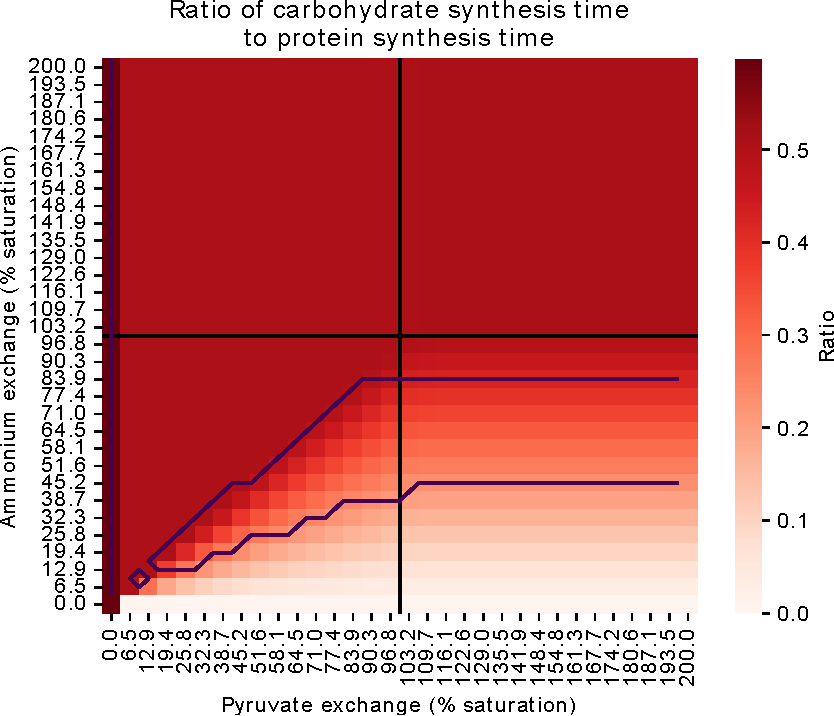
\includegraphics[width=\linewidth]{ec_grid_pyr_amm_carb_to_prot}
    \caption{
      $t_{\mathrm{carbohydrate}}^{\prime}/t_{\mathrm{protein}}^{\prime}$
    }
    \label{fig:model-grid-pyr-carb-to-prot}
  \end{subfigure}
  \caption{
    Effect of pyruvate ($R_{\mathrm{pyruvate}}$) and ammonium exchange rates ($R_{{\mathrm{ammonium}}}$) on various quantities.
    Exchange rates are expressed in percentages of growth saturation values shown in~\ref{fig:model-saturation}: pyruvate saturation being at \SI{4.44}{\milli\mole~\gram_{DW}^{-1}~\hour^{-1}} and ammonium saturation being at \SI{1.00}{\milli\mole~\gram_{DW}^{-1}~\hour^{-1}}.
    Black straight lines indicate saturation values.
    Contours show region in which ratio $r > 1$.
  }
  \label{fig:model-grid-pyr}
\end{figure}

On the gradients...
\begin{itemize}
  \item Explanation: The gradients of growth rate at each pixel in~\ref{fig:model-grid-glc-growthrate} with respect to horizontal (glucose exchange) and vertical (ammonium exchange) axes were computed.
        The heatmap shows the matrix of the magnitude of gradients of growth rate with respect to glucose exchange subtracted by the corresponding matrix with respect to ammonium exchange.
        Positive values (indigo) show a greater-magnitude glucose-axis gradient, thus indicating glucose-limiting conditions.
        Negative values (beige) show a greater-magnitude, thus indicating ammonium-limiting conditions.
  \item This seems to divide the space into C-limited growth rate, N-limited growth rate, and neither-limited growth rate.
  \item Where $r > 1$ seems to correspond to the boundary between the C-limited and N-limited regions.
  \item Growth rate near max, i.e.\ C/N not limiting: when glucose or ammonium exchange increases (there is an additive effect), temporal partitioning is more advantageous.
  \item In the N-limiting region (beige): as ammonium exchange increases, growth rate ($\lambda_{0}$) increases (decreasing $B$) and $t_{\mathrm{protein}}$ decreases (implying increasing $\lambda_{\mathrm{protein}}^{\prime}$).
        Because $r$ increases, this means that the increase in $\lambda_{0}$ `overpowers' the increase in $\lambda_{\mathrm{protein}}^{\prime}$ [SPACE FOR SOME MATHS?].
  \item In the C-limiting region (purple): as glucose exchange increases, growth rate ($\lambda_{0}$) increases (decreasing $B$) and $t_{\mathrm{carbohydrate}}$ decreases (implying increasing $\lambda_{\mathrm{carbohydrate}}^{\prime}$).
        Because $r$ stays the same, this means that the increase in $\lambda_{\mathrm{carbohydrate}}^{\prime}$ compensates for the increase in $\lambda_{0}$ [SPACE FOR SOME MATHS?].
  \item Pyruvate seems to represent an extreme case of the glucose plots.
        The main difference is with the carbon source axis -- here, the behaviour is more similar to the ammonium axis.
        This can be explained by the fact the the pyruvate saturation curve looks similar to the ammonium one.
\end{itemize}

On the C:P ratios...
\begin{itemize}
  \item The ratio > 1 part is around the boundary between C-limited growth rate and N-limited growth rate.
        So it means that if both C and N are (nearly) limiting, sequential biosynthesis is so slow that the ratio goes above 1.
  \item In the C-limited region, the C:P ratio is high (makes sense because when C is limiting, C takes long), and in the N-limited region, the C:P ratio is low (when N is limiting, P takes long).
  \item It thus makes sense that near the boundary between the regions, the C:P ratio takes intermediate values.
\end{itemize}

\section{Conclusion}
\label{subsec:model-conclusion}

% TODO: convert to prose

Interpretation of results...
\begin{enumerate}
  \item A smaller enzyme pool means that it is more advantageous for the cell to perform sequential biosynthesis of biomass components.
  \item The advantage of sequential biosynthesis of biomass components is retained in deletion strains.
  \item This balance between sequential and parallel synthesis of biomass components changes when nutrient conditions change --- particularly with carbon (glucose or pyruvate) and nitrogen (ammonium) source uptake changes.
\end{enumerate}

Discussion and relation to yeast metabolic cycle + literature...
\begin{enumerate}
  \item Results confirm temporal segregation of biosynthesis of biomass components, especially as a strategy under constraints on the size of the proteome available for the synthesis of enzymes.
        Although it is unrealistic to assume that synthesis of one class macromolecule excludes all others, this approach is still instructive as it gives a back-of-the-envelope calculation to support the notion that the cell partitions biosynthesis temporally, and gives weight to the idea that this may be one of the rationale of the existence yeast metabolic cycle.
  \item The identity of enzymes used during synthesis of biomass components may explain some experimental observations.
        It is possible that the cell synthesises carbohydrate, DNA, and RNA after one another so that usage of  oxidative phosphorylation occur at around the same time.
        This may explain cycles in dissolved oxygen concentrations.
        In addition, lipid biosynthesis often requires different enzymes than the other components, and this may explain cycling of lipid stores.
  \item Proteins are the main limiting factor for biosynthesis, mostly owing to its large mass fraction.
        This is followed by carbohydrates and lipids.
        However, the biosynthesis time varies significantly as the nutrient conditions vary.
  \item The degree of advantage of sequential biosynthesis in various conditions and the time scales predicted may explain why yeast cells perform metabolic cycling in certain nutrient conditions.
        The model however does not explain why yeast cells continue to have metabolic cycles when abruptly starved of glucose --- although a better investigation would be switching of nutrient conditions, which FBA does not offer (it only looks at steady state).

\end{enumerate}

% Upon closer inspection of the times and fluxes... [INSERT RESULTS AND DISCUSSION HERE]
% - How long does it take to replicate the genome?  It is biosynthesis of nucleotides + process of polymerising them.  There has to be super basic cell division cycle literature about this...
% - Fatty acids: cell may use pentose phosphate pathawy and gluconeogenesis to route flow in a cycle to generate masses of NAD(P)H.  Check if the fluxes suggest this.
